% !TEX root = ../main.tex
\subsection*{3.4 公司比较与财务解释：从概念关联到研究队列}\label{page:12}
\noindent\textbf{公司比较模块将产业概念转化为可以逐项审阅的研究队列。}每个公司对象同时携带证券代码、产业角色、影响方向、影响强度、风险标记、证据ID与核验状态。公司通过证券主体、产品或业务角色与图谱节点和事件路径建立显式映射；在此基础上，系统进一步刻画该公司对事件的暴露、敏感性和财务重要性。

\begin{center}
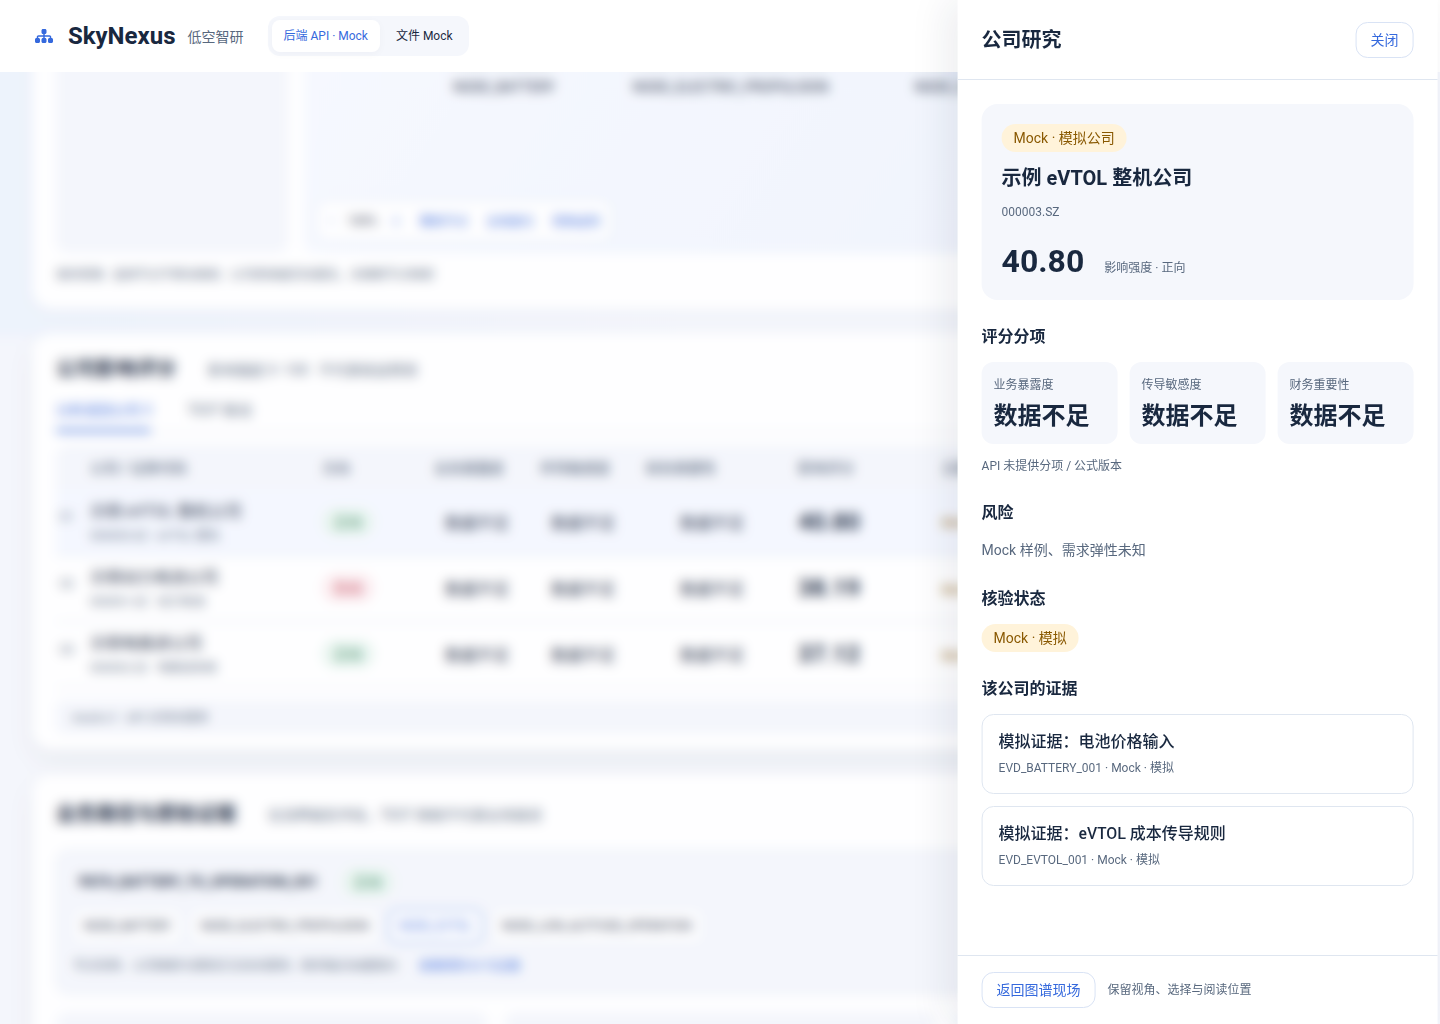
\includegraphics[width=0.90\linewidth,height=0.40\textheight,keepaspectratio]{assets/hongyulyu714-prog/fig-company-analysis.png}
\PlanFigureCaption{图12-1}{公司影响分析页面截图。页面将公司卡片、影响方向、分数、风险标记与证据入口放入同一研究现场；截图来源于\texttt{docs/screenshots/08-company.png}。图中数值属于\texttt{mock-v1}演示记录，用于展示字段和阅读路径。}
\end{center}

项目采用确定性影响强度表达式
\[
\mathrm{Impact}=\frac{\mathrm{Exposure}\times\mathrm{Sensitivity}\times\mathrm{FinancialMateriality}}{10000}.
\]
其中，\textit{Exposure}衡量公司业务与被影响产业环节的连接程度，\textit{Sensitivity}描述事件变化对该环节的传导敏感度，\textit{FinancialMateriality}表达成本、毛利、现金流或杠杆等财务变量对传导的放大程度。影响方向通过\texttt{positive}、\texttt{negative}、\texttt{neutral}和\texttt{uncertain}字段单独呈现，使研究者能够同时阅读传导方向、影响强度与风险信号\cite{lhy-scoring,lhy-architecture}。

\begin{center}\small 表12-1\quad 公司研究队列的字段、解释任务与审阅规则\par\vspace{1mm}
\begin{tabularx}{\linewidth}{p{0.20\linewidth}p{0.28\linewidth}X}
\toprule
字段组 & 回答的研究问题 & 审阅规则\\
\midrule
主体与产业角色 & 研究对象是否为明确的上市主体，位于何种业务环节？ & 使用显式证券代码和公司--产品--节点映射；概念、传闻或名称相似性不构成主体识别。\\
暴露度与敏感度 & 该公司为何会受到事件影响，影响沿何种机制传递？ & 每个参数应能追溯至产业角色、路径关系或已记录的业务事实。\\
财务重要性 & 事件传导为何可能在财务层被放大或缓冲？ & 当前为可复现代理变量；接入授权数据后按报告期、单位和口径复核。\\
方向、分数与风险 & 影响的方向、相对强度与不确定性如何共同表达？ & 方向与强度分别读取；风险标记不被压缩进单一总分。\\
证据与核验状态 & 支撑公司关联的依据是否已定位和复核？ & 证据需显式包含该证券代码；无直接关联时保留待核验状态。\\
\bottomrule
\end{tabularx}\end{center}

当前评分样例覆盖20家临时研究对象、3类事件情景和60条评分记录，并配套240条财务样例行\cite{lhy-scoring}。这些数据的作用是复现影响计算、检查单位和缺失值处理、验证前端展示，而不是替代授权财务数据库。正式比赛演示将以“公司主体可追溯、方向可解释、分数可复算、证据可定位”为评价重点，使公司比较成为研究的起点而非结论终点。
